% Introduction 

\subsection{Quantum Molecular Dynamics}
% 
The main advantage of performing quantum molecular dynamics (QMD) over classical molecular dynamics (MD) can be resumed as follwos: 1) The result is independent of the choice of the force field given that the forces are computed directly from the electronic structure of the system. 2) Allows for formation and rupture of bonds (chemical reactions) as the simulation proceeds (see figure \ref{cooh}). 3) The electronic properties of the system can be follow at each and every time step during the simulation. This is important when computing optical properties such as Raman and IR spectroscopy. 

\begin{figure}[h]
  \begin{center}  
    \begin{tikzpicture}
      \node (a) [image,yshift=0cm] {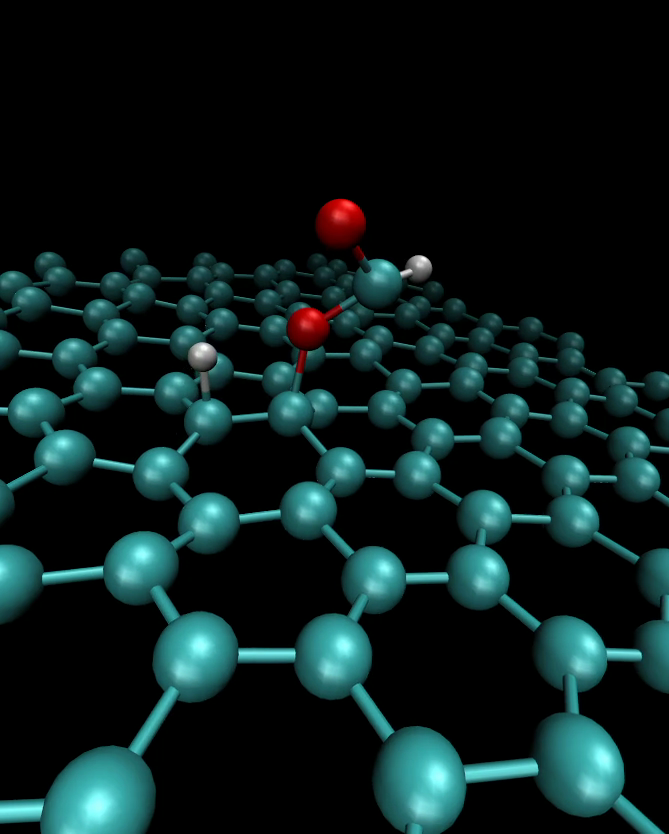
\includegraphics[width=3.0cm,trim={2cm 4cm 2cm 1cm},clip]{./fig/cooh_1.png}};
      \node (b) [right of=a, image,xshift=3cm,yshift=0cm] {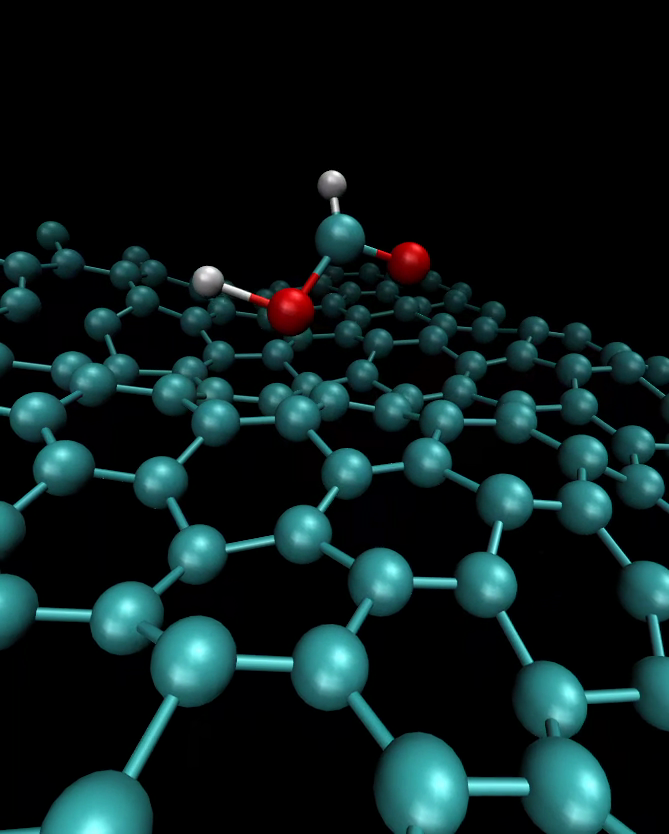
\includegraphics[width=3.0cm,trim={2cm 4cm 2cm 1cm},clip]{./fig/cooh_2.png}};      
      \draw [very thick,->] (a) to (b);
    \end{tikzpicture}    
  \end{center}
\caption{1500 K canonical QMD simulation showing the desorption of formic acid on graphene structure.} 
\label{cooh}
\end{figure}

QMD techniques will still be less computationally efficient than classical MD but with the combination of the new advances in computational sciences (new architectures) together with the techniques here described, larger system sizes and longer simulation time scales will be achieved. The (\href{https://github.com/qmmd/bml}{BML}) library, developed at LANL as part of this ECP project is helping to port the mathematical operations to the novel architectures and hence the algorithms at the \href{https://github.com/lanl/qmd-progress}{PROGRESS} library level will not need to be reformatted giving a long term maintenance of the codes. The techniques mentioned here are available in the format of libraries that are released as open source codes under BSD licenses. This libraries can be downloaded from \href{https://qmmd.github.io/}{https://qmmd.github.io/}. Figure \ref{scheme} shows a scheme on how the libraries are called from the application code. 

The QMD algorithm section of the codesignd center for particle applications (COPA) of the Exascale computing project (ECP) aims
at developing exascale optimized algorithm to compute the electronic structure within localized atomic orbitals based methods.
This set of general solvers will be in a first step optimized by constructing proxy apps. The algorithms will be further ported to 
the PROGRESS library for application into existing codes such as LATTE and DFTB+. These set of tools will be key to advance QMD towards larger systems for longer simulation timescales. 




